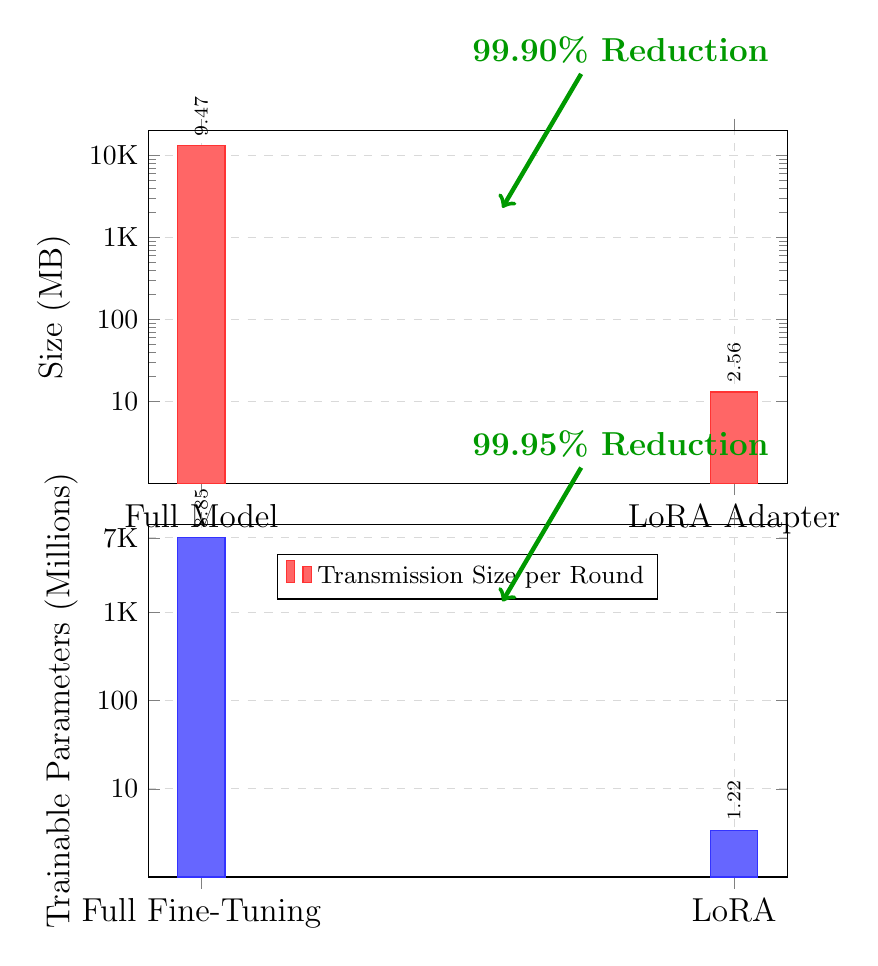
\begin{tikzpicture}
    \begin{axis}[
        ybar,
        bar width=0.6cm,
        ylabel={Size (MB)},
        ylabel style={font=\large},
        symbolic x coords={Full Model, LoRA Adapter},
        xtick=data,
        xticklabel style={font=\large},
        ymode=log,
        ymin=1,
        ymax=20000,
        ytick={10, 100, 1000, 10000},
        yticklabels={10, 100, 1K, 10K},
        legend style={at={(0.5,-0.2)}, anchor=north, legend columns=1, font=\small},
        width=0.8\textwidth,
        height=0.5\textwidth,
        grid=major,
        grid style={dashed, gray!30},
        nodes near coords,
        every node near coord/.append style={font=\scriptsize, rotate=90, anchor=west},
        ]
        
        \addplot[fill=red!60, draw=red!80] coordinates {
            (Full Model, 13000)
            (LoRA Adapter, 13)
        };
        
        \legend{Transmission Size per Round}
    \end{axis}
    
    % Add annotation
    \node[font=\large, text=green!60!black] at (6, 5.5) {\textbf{99.90\% Reduction}};
    \draw[->, ultra thick, green!60!black] (5.5, 5.2) -- (4.5, 3.5);
    
    % Trainable parameters comparison
    \begin{scope}[shift={(0,-5)}]
        \begin{axis}[
            ybar,
            bar width=0.6cm,
            ylabel={Trainable Parameters (Millions)},
            ylabel style={font=\large},
            symbolic x coords={Full Fine-Tuning, LoRA},
            xtick=data,
            xticklabel style={font=\large},
            ymode=log,
            ymin=1,
            ymax=10000,
            ytick={10, 100, 1000, 7000},
            yticklabels={10, 100, 1K, 7K},
            width=0.8\textwidth,
            height=0.5\textwidth,
            grid=major,
            grid style={dashed, gray!30},
            nodes near coords,
            every node near coord/.append style={font=\scriptsize, rotate=90, anchor=west},
            ]
            
            \addplot[fill=blue!60, draw=blue!80] coordinates {
                (Full Fine-Tuning, 7000)
                (LoRA, 3.4)
            };
            
        \end{axis}
        
        \node[font=\large, text=green!60!black] at (6, 5.5) {\textbf{99.95\% Reduction}};
        \draw[->, ultra thick, green!60!black] (5.5, 5.2) -- (4.5, 3.5);
    \end{scope}
\end{tikzpicture}
